
\documentclass[forests,article,submit,moreauthors,pdftex]{Definitions/mdpi} 
%=================================================================
\firstpage{1} 
\makeatletter 
\setcounter{page}{\@firstpage} 
\makeatother
\pubvolume{xx}
\issuenum{1}
\articlenumber{5}
\pubyear{2019}
\copyrightyear{2019}
%\externaleditor{Academic Editor: name}
\history{Received: date; Accepted: date; Published: date}
%\updates{yes} % If there is an update available, un-comment this line

%% MDPI internal command: uncomment if new journal that already uses continuous page numbers 
%\continuouspages{yes}


% \usepackage{microtype} % Slightly tweak font spacing for aesthetics
% \usepackage{amsmath, amssymb}
% \usepackage[english]{babel} % Language hyphenation and typographical rules
% \usepackage{graphicx}
\graphicspath{{img/}}
% \usepackage{float, lineno}
\usepackage{subfigure}
\usepackage{multirow}
\usepackage{adjustbox}
\usepackage{pdflscape}
\usepackage{tabularx}
\newcommand\setrow[1]{\gdef\rowmac{#1}#1\ignorespaces}
% \usepackage{tikz}
\usetikzlibrary{shapes,shadows,arrows, positioning, fit, calc, arrows.meta, shapes.geometric}
% \usepackage{algorithm}
% \usepackage{algpseudocode}
% \usepackage{longtable}
% \usepackage{titlesec}
       
\usepackage[toc, page]{appendix}

\usepackage{booktabs} % Horizontal rules in tables
% \newcommand*\bigcdot{\mathpalette\bigcdot@{.5}}
% \DeclareMathOperator{\E}{\mathbb{E}}

%----------------------------------------------------------------------------------------
%	TITLE SECTION
%----------------------------------------------------------------------------------------


% Full title of the paper (Capitalized)

\Title{Multistage Sample Average Approximation for Harvest Scheduling under Climate Uncertainty}

% Author Orchid ID: enter ID or remove command
\newcommand{\orcidauthorA}{0000-0002-1178-3229} % Add \orcidA{} behind the author's name
%\newcommand{\orcidauthorB}{0000-0000-000-000X} % Add \orcidB{} behind the author's name

% Authors, for the paper (add full first names)
\Author{Martin B. Bagaram $^{1,2^*}$\orcidA{}, S\'andor F. T\'oth $^{1}$}

% Authors, for metadata in PDF
\AuthorNames{Martin B. Bagaram,  S\'andor F. T\'oth}

% Affiliations / Addresses (Add [1] after \address if there is only one affiliation.)
\address{%
$^{1}$ \quad School of Environmental and Forest Sciences, University of Washington, Box 352100, Seattle, WA 98195, USA\\
$^{2}$ \quad Industrial and Systems Engineering, University of Washington, Seattle, WA 98195-2650, USA}

% Contact information of the corresponding author
\corres{Correspondence: martb@uw.edu}

% Current address and/or shared authorship
% \firstnote{Current address: Affiliation 3} 
% \secondnote{These authors contributed equally to this work.}


%% use optional labels to link authors explicitly to addresses:
%% \author[label1,label2]{}
%% \address[label1]{}
%% \address[label2]{}

% \author{}
% \author[a]{Martin B. Bagaram }
% \author[a]{S\'andor F. T\'oth}
% \address[a]{School of Environmental and Forest Sciences, University of Washington, Box 352100, Seattle, WA 98195, USA}
% \address[b]{Industrial and Systems Engineering, University of Washington, Seattle, WA 98195-2650, USA}


\abstract{
Forest planners have traditionally  used expected growth and yield coefficients to predict future merchantable timber volumes.
However, because climate change affects forest growth, the typical forest planning methods using expected value of forest growth can lead to sub-optimal harvest decisions.
We proposed in this paper to formulate the harvest planning with growth uncertainty due to climate change problem as a multistage stochastic optimization problem and use sample average approximation (SAA) 
as a tool for finding the best set of forest units that should be harvested in the first period even though we have a limited knowledge of what future climate will be. The objective of the harvest planning model is to maximize the expected value of the net present value (NPV) considering the uncertainty in forest growth and thus in revenues from timber harvest. The proposed model was tested on a small forest with 89 stands  and the numerical results showed that the approach allows to have superior solutions in terms of net present value and robustness in face of different climate scenarios  compared to the approach using the expected growth and yield. 
The SAA methods requires to generate samples from the distribution of the random parameter. Our results suggested that a sampling scheme that focuses on generating high number of samples in distant future stages is favorable compared to having large sample sizes for the near future stages. 
Finally, we demonstrated that, depending on the level of forest growth change,  ignoring this uncertainty can negatively affect forest resources sustainability.  
}

% %%Graphical abstract
% \begin{graphicalabstract}
% %\includegraphics{grabs}
% \end{graphicalabstract}

% %%Research highlights
% \begin{highlights}
% \item Research highlight 1
% \item Research highlight 2
% \end{highlights}

\keyword{
data-driven optimization; climate change; harvest planning; optimality gap; forest}

% \linenumbers



%----------------------------------------------------------------------------------------
\begin{document}

%%%%%%%%%%%%%%%%%%%%%%%%%%%%%%%%%%%%%%%%%%%%%%%%%%%%%%%
%%%%%%%%%%%%% TIKZ COMMANDS
\tikzstyle{vertex} = [circle, draw,  radius=3pt, very thick, font=\scriptsize]
\tikzstyle{arc} = [draw, -latex', very thick]
\tikzstyle{elli} = [ellipse, draw, dashed, color=red!50]
\tikzstyle{dot} = [draw, dotted, thick]
% \newcommand\gauss[2]{1/(#2*sqrt(2*pi))*exp(-((x-#1)^2)/(2*#2^2))} % Gauss function, parameters mu and sigma

\section{Introduction}
Climate change is arguably one of the most challenging issues that contemporary forest planners need to address. In general, forest practitioners need to provide a long term forest  harvest scheduling plan that takes into account the preference of the stakeholders while  complying with environmental, regional and ecological restrictions. Usually, forest planning aims at scheduling which forest units should receive a specific treatment such as harvesting, thinning, etc., in each period in order to achieve the management objectives. This  planning also known as harvest scheduling,  expands several decades, and is subject to many sources of uncertainties due to factors that include natural hazards (fire, windthrow, insects, etc), and  technological limitation such as forest inventory errors, growth prediction errors, poor foresight of the price of forest products on the market \citep{Makinen2013, Ross2016}. It is important to incorporate all or some of these uncertainties in forest planning.
% The uncertainty in forest planning can be addressed through a particular class of mathematical programming known as stochastic programming. 
% One can make a distinction between two-stage stochastic programming which is a type of modeling where a decision is made, then the uncertainty is revealed and a recourse action is taken, and multi-stage stochastic programming where the sequence of decision and uncertainty revealing itself occurs more than once. Multistage stochastic programming is more common in forest planning under uncertainty because of the long planning horizon in strategic harvest scheduling and the presence of relationships between decisions taken in different time periods.

The need to incorporate uncertainty in forest harvest scheduling has been acknowledged  several decades ago \citep{Dixon1980}.  Subsequently, \cite{VanKooten1992} urged for consideration of forest growth uncertainty in the planning. The authors asserted that the cost of ignoring such uncertainty at a forest scale can be detrimental.  When the uncertainty is ignored, we make decisions assuming the growth in the future will be the expected value of growth (average growth). However, it is rare that the actual growth will be the average one and therefore, many harvest decisions made in early periods of the planning horizon were not optimal. This leads to a failure to meet the planning objectives and satisfying many of the aforementioned  restrictions.
Owing to the computational challenges that the introduction of uncertainty in harvest modeling involves,  \cite{Pukkala1998}  recommended that each forest harvest scheduling plan should be accompanied by an estimation  of its uncertainty or its reliability. 
Notwithstanding all the exhortation to incorporate uncertainty in forest planning, harvest scheduling models, for a long time, have ignored uncertainty or were limited at reporting the sensitivity of the harvesting plans in case of change of one or many  input parameters of the modeling.
It is only recently that there has been a prolific number of papers addressing the integration of uncertainty in harvest planning. The most common uncertainty that has been addressed is the wood price and  demand uncertainties \citep{Alonso-Ayuso2011a, Veliz2014,Piazza2014, Pagnoncelli2017, Alonso-Ayuso2018}. Recently, there is an interest to incorporate climate uncertainty in forest planning. The first study that we are aware of that explicitly addresses the issue was conducted by \cite{Garcia-Gonzalo2016}. The authors assessed how climate change affected the management decisions of a Eucalyptus forest in Portugal with a planning horizon of 15 years. 
A similar study was conducted  by \cite{Alvarez-Miranda2018, Garcia-Gonzalo2020} using the same dataset.

In this paper, we model harvest planning as a stochastic optimization problem and use sample average approximation (SAA) as a tool for identifying the best set of actions one can take to meet the management objectives. In other words, we use SAA for solving harvest planning models. Stochastic optimization is a modeling framework for optimization problems dealing with uncertainty. 
In multistage stochastic programming, decisions are made sequentially at stages and the uncertainty unfolds during periods. Thus, the decision maker needs to implement a decision at the beginning of the planning horizon (first stage decisions) without knowing what the value of the uncertain parameter will be. After a period, in which the uncertainty is revealed, the decision maker can take recourse actions at subsequent stages. 
Therefore, it is important  to make optimal decisions in the early stages of the planning without knowing the magnitude  of the  uncertainty that will unfold. Specifically, in strategic harvest scheduling, the decision maker needs to prioritize the set of forest units (stands) that should be harvested here and now or during the ongoing decade or period. After that period, the decision maker will have the opportunity to revisit the management in the following periods. In this case, the goal of the harvest scheduling is to decide the set of actions that managers should apply immediately ``here and now" (first stage decisions). 
% This realization makes the problem suitable for sample average approximation (SAA).

SAA  is a Monte Carlo simulation based  approach for solving stochastic optimization problems. It consists of drawing repetitively  samples from the distribution of the random parameter and solving the resultant average sample deterministic optimization problem. Each sample might lead to a different solution. However, if the sample size is large enough, the sample objective function value will approximate the true optimal value. 
\cite{Mak1999} showed that for minimization problems, the expectation of samples' objective value corresponds to the lower bound on the true optimal value of the stochastic optimization problem and that the bound monotonically increases as the sample size increases. SAA has been successfully applied in several fields such as portfolio selection \citep{Wang2008}, supply chain network design  \citep{Schutz2009, Chunlin2012}, facility location problem \citep{Emelogu2016}  and personnel assignment \citep{Pour2017}.
Notwithstanding all these applications, and the fact that SAA is  well suited for problems where the objective function is difficult to evaluate such as harvest planning under climate uncertainties \citep{Wang2008}, to the extent of our knowledge, SAA has never been applied  in forestry domain. In addition, unlike  stochastic programming which requires to know the probability distribution of the samples, SAA known as a data-driven optimization method,  considers the samples to be equiprobable. The idea is that if the sample size is large enough, then the sample statistics will represent those of the actual population the sample is taken from. Hence, there is no need to know the actual distribution of the uncertainty.
This is particularly important for harvest scheduling under climate uncertainty because climate change is forecast as possible futures without any probabilities. Moreover, although the method performs well for two-stage stochastic problems \citep{MohammadiBidhandi2017}, it is unclear how the method will perform on a multistage harvest scheduling problem.
% correlation among random parameters in different stages of multistage programming should be handled.

The objective of this paper is to fill the gap in the literature on SAA and multistage stochastic harvest scheduling models. For multistage stochastic optimization problems, each sample of the uncertainty is known as a scenario. It is known that the number of scenarios to consider grows exponentially with the number of stages in multistage stochastic programs. Forest harvesting scheduling models are typically characterized with long planning horizons with many stages. The contributions in this paper are as follows:

\begin{enumerate}
    \item Introduce a method to handle climate change uncertainty in forest harvest scheduling that allows to make sound decisions in early stages of  planning. Poor decisions in early stages are significantly more detrimental to many businesses compared to decisions in later stages. Hence,  later stage decisions can be considered as secondary. 
    % We achieve this objective by extending SAA to harvest scheduling with forest growth under climate uncertainty. Stochastic harvest scheduling under climate uncertainty problems have uncertainty in both the constraints and the objective function.
    \item Propose a method to generate the set of scenarios to reduce the sample size and keep the optimization model tractable. If we generate possible scenarios of forest growth in i.i.d (independent identical distributed) fashion, then we might have a very large sample size before SAA solution converges to optimality. This large sample size can make the problem computationally intractable. 
    We propose a sampling scheme that focuses at having higher number of replications for distant stages.
\end{enumerate}  
We will show that  stochastic harvest scheduling has an advantage over the expected value approach (deterministic model presented in Appendix \ref{app:det_harv}) because it allows to implement policies that are optimal for all foreseen forest growth change by providing management decisions that would be implemented if we consider the uncertainty and if we do not. The rest of this document is structured as follows. In Section \ref{sec:material_methods}, we present the materials and methods used in this research. We describe in that section the SAA method and the scenario generation scheme. We dedicate Section \ref{sec:num_res} to presenting our findings. Finally, in Section \ref{sec:conclusion}, we discuss the results and outline future research.

\section{Material and methods} \label{sec:material_methods}
% \subsection{Deterministic}

\subsection{Problem description and formulation} \label{sec:prob_descr}

We present in this section the multistage stochastic harvest scheduling problem with forest growth uncertainty due to climate change. Let $ t \in \mathcal{T}=\{1,\dots, T\}$ be the set of stages in which forest units are eligible for harvest in the future. We reserve $t=0$ to the time ``now" (first stage decision), where there is no uncertainty on the forest growth. We define $\xi := \{ \xi_1, \dots, \xi_T \}$ to be the random vector characterizing forest growth change due climate change. Hence, $\xi_t$ is the random parameter of $\xi$ at time $t$. Each $\xi_t$ has a support  $\Xi_t$ which is the range of values that the random parameter $\xi_t$ can take. 
The meaning of parameters, variables and sets is given in Table \ref{tb:harv_param}.

The objective of the decision maker is to maximize the expected net present value (NPV) from timber harvest. This can be formulated in a generic form as (\ref{eq:obj_1_}) and (\ref{eq:def_x}):
\begin{align}
    & \max \; \sum_{s \in \mathcal{S}}r_{s} x_{s} + \operatorname{\mathbb{E}}\Big[ R(x, \xi) \Big] \label{eq:obj_1_}\\
& \text{subject to} \quad
 x \in \{0, 1\}^{|\mathcal{S}|}, \label{eq:def_x}
\end{align}
where we take the expectation with respect to $\xi$ and,  $ R(x, \xi^{i})$ is the optimal value of the harvest scheduling given the harvest in the first stage ($x$) and the occurrence of one climate scenario $\xi^i$. In this formulation, the decision variables are only the first stage variables which means that the decision maker mainly cares about how to select the stands that can be harvested in the first period so that the expected NPV is maximized. 
The value of $ R(x, \xi^{i})$ is obtained by solving the following optimization problem:

\begingroup
% \allowdisplaybreaks
\begin{align}
    & \max \; \sum_{s\in \mathcal{S}} \Bigg[ \sum_{t\in \mathcal{T}} r^{\xi^{i}}_{st}y_{st}^{\xi^{i}}  + r^{\xi^{i}}_{s0} w_s^{\xi^{i}} \Bigg]\label{eq:obj_2_}\\
& \text{subject to} \nonumber\\
    &  x_s + w_s^{\xi^{i}} + \sum_{t=1}^T y_{st}^{\xi^{i}} = 1 &&  s=1,\dots, |\mathcal{S}| \label{eq:one_harvest}\\
    & \sum_s v_s x_s  = H_0 \label{eq:compute_v0}\\
    & \sum_s v_{st}^{\xi^{i}} y_{st}^{\xi^{i}} = H_{t}^{i} &&  t = 1, \dots, T \label{eq:compute_v_others}\\
    & H_t^{i} \le \alpha H_{t-1}^{i} &&   t=1, \dots, T \label{eq:vol_flu_low}\\
    & H_t^{i} \ge \beta H_{t-1}^{i} &&  t=1, \dots, T \label{eq:vol_flu_high}\\
     & H_t^{i} \le \gamma H_{t-2}^{i} &&   t=2, \dots, T \label{eq:vol_flu_low2}\\
    & H_t^{i} \ge \lambda H_{t-2}^{i} &&  t=2, \dots, T \label{eq:vol_flu_high2}\\
    & \sum_{s\in \mathcal{S}}a_s\Bigg[\sum_{t=1}^{\mathcal{T}} age_{st}(x_{s} + y_{st}^{\xi^{i}}) + age_{s0}w_{s}^{\xi^{i}}\Bigg] \ge \sum_s a_s age_{s.} \label{eq:age_end}\\
    & w^{\xi^{i}} \in \{0, 1\}^{|\mathcal{S}|}, \; \; y^{\xi^{i}} \in \{0, 1\}^{|\mathcal{S}| \times T}, \; \; H_{t}^{i} \ge 0 && \forall t \in \{0, 1, \dots, T\}. \label{eq:var_definition}
\end{align}
\endgroup

\begin{table}[hbtp!]
    \caption{Variable, set and parameters used in problem formulation}
    \label{tb:harv_param}
    \centering \small
    \begin{tabularx}{\linewidth}{lX}
\textbf{Sets}\\
     $\mathcal{S}$ & set of stands or forest management units ($s\in \mathcal{S}$)\\
     $\mathcal{T}$ & set of time period in which the decision are implemented  or stage at which the decisions are taken ($t \in \mathcal{T}$)\\
     $\Omega$ & set of scenarios ($\xi^{i} \in \Omega$)\\
% \textbf{Indices}\\
%     $s$ & stand ID or forest management unit ID ($s\in \mathcal{S}$).\\
%     $t$ & time period in which the decision are implemented  or stage at which the decisions are taken ($t \in \mathcal{T}$)\\
%     $\xi^{i}$ & scenario i with $\xi^{i} \in \Omega$\\
%     % $\omega, \omega^{\prime}$ & scenario\\
\textbf{Variables}\\
    $x_{s}$ & binary variable: 1 if management unit  $s$ is scheduled to be harvested in the first period (now); and 0 otherwise\\
    % $z_{st}$ & binary: 1 if   management unit  $s$ has been harvested before the current management such that the stand is not green-up yet at time t; and 0 otherwise. It is not an actual variable since it is defined while building the model\\
    $w_{s}^{\xi^{i}}$ & binary variable: 1 if  management unit $s$ should not be harvested during the whole planning horizon given the scenario $\xi^{i}$; and 0 otherwise\\
    $y_{st}^{\xi^{i}}$ & binary variable: 1 if the stand $s$ should be harvested in $t$ given the scenario $\xi^{i}$; 0 otherwise \\
     $H^i_t$ &  volume harvested in year $t$ under scenario $\xi^i$ ($m^3$).   We omit the superscript $i$ for $t=0$\\
\textbf{Parameters}\\
     $r_s$ & discounted net harvest revenue from stand $s$ if the stand is harvested now (\$)\\
     $r^{\xi^{i}}_{st}$ & net harvest revenue from stand $s$ if the stand is harvested in year $t$ according to scenario $\xi^i$ (\$)\\
     $r^{\xi^{i}}_{s0}$ & discounted value of the stand at the end of the planning horizon if it is not harvested during the whole planning horizon under scenario $\xi^i$ (\$)\\
     $v_{s}$ & merchantable yield of stand   $s$  in the first period ($m^3/ha$)\\
     $v_{st}^{\xi^{i}}$ & projected merchantable yield of  stand $s$ if harvested in year $t$ according to scenario $\xi^{i}$ ($m^3$/ha)\\
     $a_s$ & area of stand $s$ (ha)\\
     $age_{st}$ & age of stand $s$ at the end of the planning horizon if harvested in year $t$ (yr)\\
     $age_{s.}$ & current age of the stand $s$ (yr)\\
     $age_{s0}$ & age of stand $s$ at the end of the planning if not harvested during the planning horizon (yr)\\
     $\alpha$ & acceptable lower bound on the fluctuation of volume of wood from one period to the next\\
     $\beta$ & acceptable upper bound on the fluctuation of volume of wood from one period to the next\\
     $\gamma$ & acceptable lower bound fluctuation of volume of wood between two non consecutive periods\\
     $\lambda$ & acceptable upper bound fluctuation of volume of wood between two non consecutive periods\\
\end{tabularx}
\end{table}

The objective function (\ref{eq:obj_2_})  maximizes the net present value from subsequent stages after the current harvest ($x$). This objective function includes the cost of harvest and re-plantation for each forest unit. In addition, this objective function accounts for the value of the stands that are not harvested during the planning horizon because those stand have a monetary value. Constraint set (\ref{eq:one_harvest}) imposes that if a stand is harvested now, then it cannot be harvested in subsequent years. In other words a forest unit can only be harvested once during the whole planning horizon. The use of $w_s$ variables is to account the stands that are not scheduled for harvest in the whole planning horizon.
Constraint set (\ref{eq:compute_v0}) and (\ref{eq:compute_v_others})  compute the volume of wood harvested  now and in the future periods during the planning horizon, respectively. The volume computed in each period depends on the scenario $\xi^i$.
Constraint sets  (\ref{eq:vol_flu_low}) and  (\ref{eq:vol_flu_high}) impose that the volume fluctuation between two consecutive stages should be within a given lower and upper bounds, respectively. These set of constraints are also known as even flow constraint since they ensure that the volume of timber harvested is almost evenly distributed in time. Even with constraint sets  (\ref{eq:vol_flu_low}) and  (\ref{eq:vol_flu_high}), there is a possibility that the volume harvested declines with time. Hence volume at $t=4$ might be much lower than volume at $t=1$, for instance. To attenuate this effect, we impose supplementary wood flow constraints which are constraint sets (\ref{eq:vol_flu_low2}) and  (\ref{eq:vol_flu_high2}). These two sets of constraints impose flow restriction between two non-consecutive stages.
Constraint set (\ref{eq:age_end}) states that the age of the forest at the end of the planning horizon should be greater or equal to the current age of the forest. 
% In the constraint, when $t=0$, $y_{st}=0$. 
This constraint is a proxy for sustainability; it ensures that forest resources are not depleted during the planning horizon.  Finally, the definition of the variables is given in (\ref{eq:var_definition}).

% In sum, the whole formulation can be written as 
% \begin{align}
%     & \max \; \sum_{s \in \mathcal{S}}r_{s} x_{s} + \sum_{\xi^{i} \in \Omega}\rho^{i}\Bigg[\sum_{s\in \mathcal{S}} \Big( \sum_{t\in \mathcal{T}} r^{\xi^{i}}_{st}y_{st}^{\xi^{i}}  + r^{\xi^{i}}_{s0} w_s^{\xi^{i}} \Big)\Bigg]\\
% & \text{subject to constraints \eqref{eq:def_x}, \eqref{eq:one_harvest} to \eqref{eq:var_definition}} \quad \forall\; \xi^{i} \in \Omega
% \end{align}
% where $\rho^{i}$ is the probability of the scenario $\xi^{i}$.
% \subsection{Climate data and multistage sampling}
\subsection{Climate change data}

In this paper the uncertainty in forest growth stems from climate change. We present in this section how climate change was translated into forest growth to be suitable to the harvest planning model.
Climate change in this project refers to the change in forest growth. Hence, the change can be positive or negative. The change is small in near future, stage 1, compared to the distant future (stage 4). There is a ten year difference between two consecutive stages. 
In this project, we consider the case of Pacific Northwest where most models forecast that climate change will lead to the increase of forest growth. We report in Table \ref{tb:climate_data} the growth change used for the analysis. This growth change data is based on \cite[Table 3]{Latta2010}. Forest growth is age dependent and this is reflected in growth change. In addition, this growth change  modeling reflect a Geometric Brownian Motion process where the absolute increment of growth are not independent from one period to another although the percentages of change are.
% The first one is a mild climate change with only mild forest growth changes and the second one is a severe climate change (Table . 
% This dataset, although theoretical, mirrors the finding of. 
The \texttt{Lower} and \texttt{Upper} in the table correspond to the lowest and highest possible growth change, respectively, at each stage. 
Formally speaking, [\texttt{Lower}, \texttt{Upper}] at stage $t$, represents $\Xi_t$ of the random parameter $\xi_t$.

To assess the performance of the proposed modeling framework, we change the lower bound on the growth change by multiplying it by a factor $\epsilon$. This allows to assess the performance of the proposed method for climate change scenarios that forecast decrease in forest growth. We assessed values of $\epsilon$ equal 1, 20 and 40. Only $\epsilon = 40$ corresponds to forest decline whereas, $\epsilon$ of  20 corresponds to a decrease in forest growth.

\begin{table}[!htb]
\caption{Forest growth change (\%) due to climate change}
\label{tb:climate_data}
\centering
\adjustbox{max width=\linewidth}{
\begin{tabular}{crrrr}
\toprule
% \multicolumn{1}{l}{}      & \multicolumn{2}{l}{Mild  change}                      & \multicolumn{2}{l}{Severe change}                     \\
% \midrule
\multicolumn{1}{c}{Stage} & \multicolumn{1}{c}{Lower} & \multicolumn{1}{c}{Upper} \\ \hline
1                         & -1.2                        & 11.1                                               \\
2                         & -2.4                        & 22.2                                                 \\
3                         & -3.6                        & 33.3                                                 \\
4                         & -4.8                      & 44.4                       &  \\    
\bottomrule
\end{tabular}
}
\end{table}

\subsection{Multistage sampling} \label{sec:sampling}

We have presented both the optimization model  we intend to solve in this paper and the uncertain parameter. In this section, we describe how to sample from the distribution of the uncertain parameter. To achieve that objective,  let $\mathcal{N} = \{N_1, \dots, N_{T} \}$ be a sequence of positive integers. At the first stage (stage 1), we generate $N_1$ replications drawn from $\Xi_1$, the support of the random parameter $\xi_1$. To minimize the number of replications necessary, we generate the $N_1$ by diving  $\Xi_1$ into $N_1$ intervals. From each interval, we sample uniformly one realization of $\xi_1$. We repeat this procedure for stage 2 and so forth for the following stages. At the end, we connect the realization at $t=0$ to all realizations at $t=1$. We connect all realizations at $t=1$ to all others at $t=2$ and we continue until the last stage. The result of this procedure is a scenario tree with a total number scenarios or sample size  $n = \prod_{t=1}^{T}N_t$. Each path from this scenario tree can be viewed as a scenario with probability $1 / n$. Varying the values of $N_t$ allows to have different sample sizes which can be solved using SAA as described in the following section. It is not clear, however, whether having $N_1 \ge N_2 \ge \dots \ge N_T$ is preferable to a sampling scheme with $N_1 \le N_2 \le \dots \le N_T$. To answer  this question, we tested the solution by considering a sampling scheme with  $N_1 = N_2 =\dots = N_T$ in Section \ref{sec:sampl_size_effect} and evaluate in Section \ref{sec:sampl_scheme}, the solution behavior when we use the two other sampling schemes.

\subsection{Solution method}
We used SAA as the method for solving the stochastic harvest scheduling model since the main challenge of the decision maker is to find the set of stands that are suitable for harvest in the first period. SAA method is a Monte Carlo simulation based  approach for solving stochastic optimization problems. A random sample is generated with uniform probability distribution, and then the expected value function of the stochastic problem is approximated by the corresponding sample average function. The sample average approximation problem which is specified by the generated sample is then solved by a deterministic optimization technique which is mixed integer programming in this study. This procedure is repeated by increasing the  size of the samples to obtain solutions that are close enough to the true optimal solution.
% Define block styles
\tikzstyle{decision} = [diamond, draw, fill=blue!20, 
    text width=3.5em, text badly centered, node distance=3cm and 7cm, inner sep=0pt]
\tikzstyle{block} = [rectangle, draw, draw=blue, fill=green!20,  thick, 
    text width=12em, text centered, rounded corners, minimum height=2.em, node distance=1.1cm]
\tikzstyle{line} = [draw, -latex']
\tikzstyle{stepz} =[fill=white, text=black, rectangle, text width=.5em, align=right, rounded corners]


To formally introduce the SAA method we used to solve the harvest scheduling problem, we reformulate the harvest scheduling problem  in \eqref{eq:obj_1_} and \eqref{eq:def_x} in a compact form, just for practicability. We can rewrite the problem as
\begin{align}
    & \max_{x \in X} \; f(x, \xi) := \max_{x \in X} \operatorname{\mathbb{E}}\Bigg[ \sum_{s \in \mathcal{S}}\big[r_{s} x_{s}\big] + R(x, \xi) \Bigg], \label{eq:reformulation}
\end{align}
where $X$ is the feasible set (constraints \eqref{eq:def_x}, \eqref{eq:one_harvest} to \eqref{eq:var_definition}). We can write (\ref{eq:reformulation}) because the term $r_{s} x_{s}$ has no uncertainty.

Let $\xi^1, \dots, \xi^n$ be a sample of size $n$ drawn from the distribution of $\xi$. The sample is generated using the method described in Section \ref{sec:sampling}. We can write the sample average objective function as: 
% (\ref{eq:saa_funct}). 
\begin{align}
    f_n(x) := \frac{1}{n}\sum_{i=1}^{n} f(x, \xi^{i}). \label{eq:saa_funct}
\end{align}
where 
\begin{align}
    & f(x, \xi^{i}) = \sum_{s \in \mathcal{S}}r_{s} x_{s} + \sum_{s\in \mathcal{S}} \Big( \sum_{t\in \mathcal{T}} r^{\xi^{i}}_{st}y_{st}^{\xi^{i}}  + r^{\xi^{i}}_{s0} w_s^{\xi^{i}} \Big).
% & \text{subject to constraints \eqref{eq:def_x}, \eqref{eq:one_harvest} to \eqref{eq:var_definition}} \quad \forall\; \xi^{i} \in \Omega
\end{align}
% where $\rho^{i}$ is the probability of the scenario $\xi^{i}$.
The idea of SAA is to solve (\ref{eq:saa}) instead of (\ref{eq:reformulation})
\begin{align}
     z_n = \max_{x \in X} f_n(x) \label{eq:saa}
    %  =  \max_{x \in X}  \frac{1}{n}\sum_{i=1}^{n} f(x, \xi^{i}) 
\end{align}

\begin{figure}[hbt!]
    \centering
    \begin{tikzpicture}[thick]
    \tikzstyle{every node}=[font=\scriptsize]
%% Place nodes
    \node [block] (b_cpath) {Initialize n and N such that $N >> n$ and generate a sample of size $N$};
    \node [stepz] at (b_cpath.west) {a};
    \node [block, below of=b_cpath, yshift=-.3em] (b_dist) {solve the SAA problem with size N to obtain $\hat{x}$};
    \node [stepz] at (b_dist.west) {b};
    \node [block, below of=b_dist, yshift=-.3em] (b_nb) {Generate $M$ samples of size $n$};
    \node [stepz] at (b_nb.west) {c};
    \node [block, below of=b_nb,  yshift=-1.3em] (b_many_trees) {Solve each sample $m$ with size $n$ SAA problem to obtain
    $z_n^m = \max _{x \in X} \frac{1}{n} \sum_{i=1}^{n} f_n\left(x, \xi^{i}\right)$ and \\ the upper bound $\overline{z}_n^M=\frac{1}{M}\sum_{m=1}^{M}z_n^{m}$};
    \node [stepz] at (b_many_trees.west) {d};
    \node [block, below of=b_many_trees, yshift=-1.7em] (b_solve_scen) {Use the first stage solution $\hat{x}$ to get a lower bound on the optimal solution $\hat{z}_n^m(\hat{x})= \max \frac{1}{n} \sum_{i=1}^{n} f_n\left(\hat{x}, \xi^{i}\right)$};
    \node [stepz] at (b_solve_scen.west) {e};
    \node [block, below of=b_solve_scen, yshift=-1.3em] (b_check_stb) {Compute the average optimality gap $\overline{G}(\hat{x}) = \overline{z}_n^M - \frac{1}{M}\sum_{m=1}^{M}\hat{z}_n^m(\hat{x})$};
    \node [stepz] at (b_check_stb.west) {f};
    \node [decision, below of=b_check_stb, yshift=1.5em] (d_stable) {Is the optimality gap small enough?};
    \node [block, right of=d_stable, xshift=6.8em, text width=2.6cm] (b_increase_nb) {Increase the sample size};
    \node [stepz](g_step) at (b_increase_nb.west) {g};
    \node [block, below of=d_stable, yshift=-3.em] (b_ci) {Get the optimal solution and its statistics};
    \node [stepz] at (b_ci.west) {h};
    % \node [decision, below of=b_ci, yshift=2.5em] (d_more_cp) {Is there more climate paths?};
    % \node [block, right of=d_more_cp, xshift=11em] (b_an_path) {Select another climate path};
    % \node [stepz](i_step) at (b_an_path.west) {i};
    % \node [block, below of=d_more_cp, yshift=-2.8em] (b_swap_sol) {Check convergence of climate paths $i$ and $j$ using solution from $i$ in the tree of $j$};
    % \node [stepz] at (b_swap_sol.west) {j};
    % \node [decision, below of=b_swap_sol, yshift=2em] (d_same_val) {Are solutions from $i$ and $i$ in $j$ the same?};
    % \node [block, right of $\mu_{\hat{x}} \in \left[0, \overline{G}+t_{M-1, \alpha} S_{\overline{G}\left(M\right)}\right]$

% =d_same_val, xshift=11em] (b_same) {Terminate. The two climate paths lead to same solutions};
    % \node [stepz] at (b_same.west) {l};
    % \node [block, left of=d_same_val, xshift=-11em] (b_diff) {Create synthetic scenario tree};
    % \node [stepz] at (b_diff.west) {k};
%
    \path [arc] (b_cpath) -- (b_dist);
    \path [arc] (b_dist) -- (b_nb);
    \path [arc] (b_nb) -- (b_many_trees);
    \path [arc] (b_many_trees) -- (b_solve_scen);
    \path [arc] (b_solve_scen) -- (b_check_stb);
    \path [arc] (b_check_stb) -- (d_stable);
    \path [arc] (d_stable) -- node[yshift=1em] {no} (g_step);
    \path [arc] (d_stable) -- node[xshift=1em] {yes} (b_ci);
    % \path [arc] (b_ci) -- (d_more_cp);
    \path [arc] (b_increase_nb) |-  (b_nb);
    % \path [arc] (d_more_cp) -- node[yshift=1em] {yes} (i_step);
    % \path [arc] (b_an_path) |-  (b_nb);
    % \path [arc] (d_more_cp) -- node[xshift=1em] {no} (b_swap_sol);
    % \path [arc] (b_swap_sol) --  (d_same_val);
    % \path [arc] (d_same_val) -- node[yshift=1em] {yes} (b_same);
    % \path [arc] (d_same_val) -- node[yshift=1em] {no} (b_diff);
    % \path [dot, -latex', very thick] (b_diff) |-  (b_nb);
%
\end{tikzpicture}
    \caption{Flow chart of SAA}
    \label{fig:saa_flowchart}
\end{figure}{}

We now describe the steps for solving a stochastic optimization problem using SAA as outlined in Figure \ref{fig:saa_flowchart}.
    
\textbf{Step a \& b:} Generate a large sample of  size ($N$) and solve it using \eqref{eq:saa} to obtain a first stage candidate solution $\hat{x}$. The choice of $N$ depends on the model that can be solved in a reasonable time. The fact that this problem is only solved once partially motivates on choosing the largest possible sample size.

\textbf{Step c:} Generate $M$ samples of size $n$. The idea is to start with lower values of $n$ and increase the sample size progressively. \cite{Kleywegt2001} describes a procedure for choosing the value of $M$. In a nutshell,  $M$ should be chosen in a way that allows to compute different statistics such as the mean, variance and confidence interval.

\textbf{Step d:} Solve SAA problem of each sample $m$ to get $z_n^m =\max _{x \in X} \frac{1}{n} \sum_{i=1}^{n} f_n\left(x, \xi^{i}\right)$ and the upper bound $\overline{z}_n^M=\frac{1}{M}\sum_{m=1}^{M}z_n^m$. $\overline{z}_n^M$ is an upper bound because it is the average of upper bounds $z_n^m$ obtained by using only a set of scenarios, and therefore the solution is more optimistic.

\textbf{Step e:} For each sample $m$, fix the first stage variables to $\hat{x}$ obtained from  step a \& b to get a lower bound on the optimal solution $\hat{z}_n^{m}(\hat{x})= \max \frac{1}{n} \sum_{i=1}^{n} f_n\left(\hat{x}, \xi^{i}\right)$
 
 \textbf{Step f:} Compute the average optimality gap as $\overline{G}(\hat{x}) = \overline{z}_n^M - \frac{1}{M}\sum_{m=1}^{M}\hat{z}_n^m(\hat{x})$. We can also compute for each sample $m$ the optimality gap as 
 \begin{align}
    G_{n}^{m}(\hat{x}) = \max _{x \in X} \frac{1}{n} \sum_{i=1}^{n} f_n\left(x, \xi^{i}\right) - \frac{1}{n} \sum_{i=1}^{n} f_n\left(\hat{x}, \xi^{i}\right) \label{eq:gap}
\end{align}
where $f_n\left(\hat{x}, \xi^{i}\right)$ is obtained by fixing the first stage variable in $f_n$ to $\hat{x}$ from Step a. 
Notice that $ G_{n}^{m}(\hat{x}) \ge 0$.
We can then compute the average optimality gap $\overline{G}(\hat{x}) = \frac{1}{M}\sum_{m=1}^{M}G_n^m(\hat{x})$ and its variance $s_{\overline{G}}^{2} = \frac{1}{M(M-1)} \sum_{m=1}^{M}\left(G_{n}^{m}(\hat{x})-\overline{G}(\hat{x})\right)^{2}$.
\cite{Mak1999} proved that the optimality gap depends on the sample size $n$ . In fact, they proved that as $n \rightarrow \infty$, the optimality gap converges to zero and the SAA objective function value  converges to the true optimal objective value with probability one. In other words, the sample size is large enough if we have a small optimality gap.

 \textbf{Step g:} If the optimality gap computed in step f is not sufficiently small, then increase the sample size $n$ and go back to step c. The decision of whether the optimality gap is sufficiently small and its variance is sufficiently low is domain specific. 
 
 \textbf{Step h:} If the optimality gap is small enough,  then we have obtained the optimal solution and we can compute the confidence interval on the  optimality gap as:
 $\mu_{\hat{x}} \in \left[0, \overline{G}(\hat{x})+t_{M-1, \alpha} S_{\overline{G}}\right]$
with a confidence of $100(1-\alpha)$ with $\alpha$ being Type I error. 
 
%  Since the value of the optimality gap, $G_n(\hat{x})$, depends on the candidate solution $\hat{x}$ and the samples $\xi^i$, there is a procedure to compute the bounds on that optimality gap. We describe in this section the multiple replications procedure \citep{Morton2006} that can be used for that end.\\
 
% \adjustbox{width=.85\linewidth}{
% \begin{tabular}{l} 
% \toprule
% Multiple Replications Procedure \\
% \hline Input: Candidate solution $\hat{x}$, the number of samples $N$, \\the number of replications 
% $M_{G}$ and $\alpha \in [0,1)$ \\
% 1: for $i=1,2, \ldots, M_{G}$ do \\
% 2: Sample i.i.d observations $\xi^{i 1}, \xi^{i 2}, \ldots, \xi^{i N}$ from the distribution of $\xi$ \\
% 3: Calculate $G_{N}^{i}(\hat{x})$ using (\ref{eq:gap}) \\
% 4: end for \\
% 5: Calculate gap estimate $\overline{G}_{M_{G}}$ and variance $S_{G}^{2}\left(M_{G}\right)$ \\
% $\overline{G}_{M_{G}}=\frac{1}{M_{G}} \sum_{i=1}^{M_{G}} G_{N}^{i}(\hat{x}) \quad s_{G}^{2}\left(M_{G}\right)=\frac{1}{M_{G}-1} \sum_{i=1}^{M_{G}}\left(G_{N}^{i}(\hat{x})-\overline{G}_{M_{G}}\right)^{2}$ \\
% 6: Output the one-sided confidence interval on $\mu_{\hat{x}}$ \\
% $\qquad \mu_{\hat{x}}=\left[0, \overline{G}_{M_{G}}+\frac{t_{M_{G}-1, \alpha} S_{G}\left(M_{G}\right)}{\sqrt{M_{G}}}\right]$\\
% \bottomrule
% \end{tabular}
% }\\

% The result of the algorithm is the $100(1-\alpha)$ confidence interval on the optimality gap. 

\subsection{Importance of SAA}
To assess the advantage of solving the stochastic optimization problem with SAA instead of the deterministic model that only consider the average scenario (the model that ignores climate change uncertainty), we compute the so-called value of stochastic solution ($VSS$) \citep{Birge1982}.
Let $\Bar{x}$  be the first stage solution we would get if we implemented the average growth solution, respectively. Similarly, let $x^{*}$ be the optimal solution of the stochastic model obtained from SAA. 
We denote by $z^{i}$ and $\Bar{z}^{i}$  the net NPVs of the scenario $\xi^{i}$ when the first stage variables are fixed to $x^{*}$ and $\Bar{x}$, respectively. Finally, let $z(\Bar{x}) = \frac{1}{|\Omega|}\sum_{\xi^{i} \in \Omega}\Bar{z}^{i}$ whereas, $z(x^{*}) = \frac{1}{|\Omega|}\sum_{\xi^{i} \in \Omega} z^{i}$. We compute $VSS$ as follows:
$
    VSS = z(x^{*}) - z(\Bar{x}).   
$
In term of relative value, we present $VSS$ in basis points (bps)\footnotemark as:
\begin{align}
    VSS(bps) = \frac{ VSS}{z(\Bar{x})} * 10,000
\end{align}
\footnotetext{1 Basis points (BPS) is equivalent to 0.01\%. It is commonly used in economics and finance}
In case where some scenarios are not feasible after fixing the first stage to $\Bar{x}$, we report the number of infeasible scenarios. 
% instead of the value of the stochastic solution.

% We report $VSS$ from 30 replications.
\subsection{Experiment}

We present in this section, the values of several parameters introduced in the methods in order to conduct a numerical experiment. The numerical experiment was run on a Windows desktop with an AMD 8 Core processor of 4 GHz and 8 GB of RAM. We have used CPLEX 12.8 to solve the stochastic model using python 3 as the modeling language. We solved each model to 0.5\% mixed integer programming (MIP) optimality gap. For each model, we generated 30 independent replications ($M = 30$). We used bootstrapping to compute the 95\% confidence level for different metrics.  $N$ was set to 625 scenarios and we varied the sample size $n$ from 16 to 625.
We tested the modeling on Phyllis Leeper forest with 89 stands (\url{http://ifmlab.for.unb.ca/fmos/datasets/PhyllisLeeper/}). Model parameters $\alpha$ and $\gamma$  were set to 0.85, whereas $\beta$ and $\lambda$ were set to 1.15. The planning horizon was 50 years divided into 5 planning periods of 10 years each.

\section{Results} \label{sec:num_res}

\subsection{Effect of sample size on the optimality gap} \label{sec:sampl_size_effect}

The results of the experiments are summarized in Figure \ref{fig:saa_performance}. The sample size is the number of scenarios. These results were obtained by setting $N_1=N_2=N_3=N_4$. 
The solutions show that as the sample size increases, the NPV decreases converging toward the optimal objective function value. In addition, we have tighter confidence intervals as the sample size increases. A similar behavior is observed for the optimality gap. However, larger sample sizes lead to a significant increase in solution time.  We can conclude that solving problems with up to 256 scenarios is sufficient to capture the variability and obtain solutions that are close enough to the true optimal solution since increasing the sample size to 625 did not significantly reduce the optimality gap and its variance. Furthermore, although we need larger sample size  to reduce the optimality gap and its variance, we need to compromise on solution time. The solution time increases exponentially with the sample size.


\begin{figure}[hb!]
    \centering
    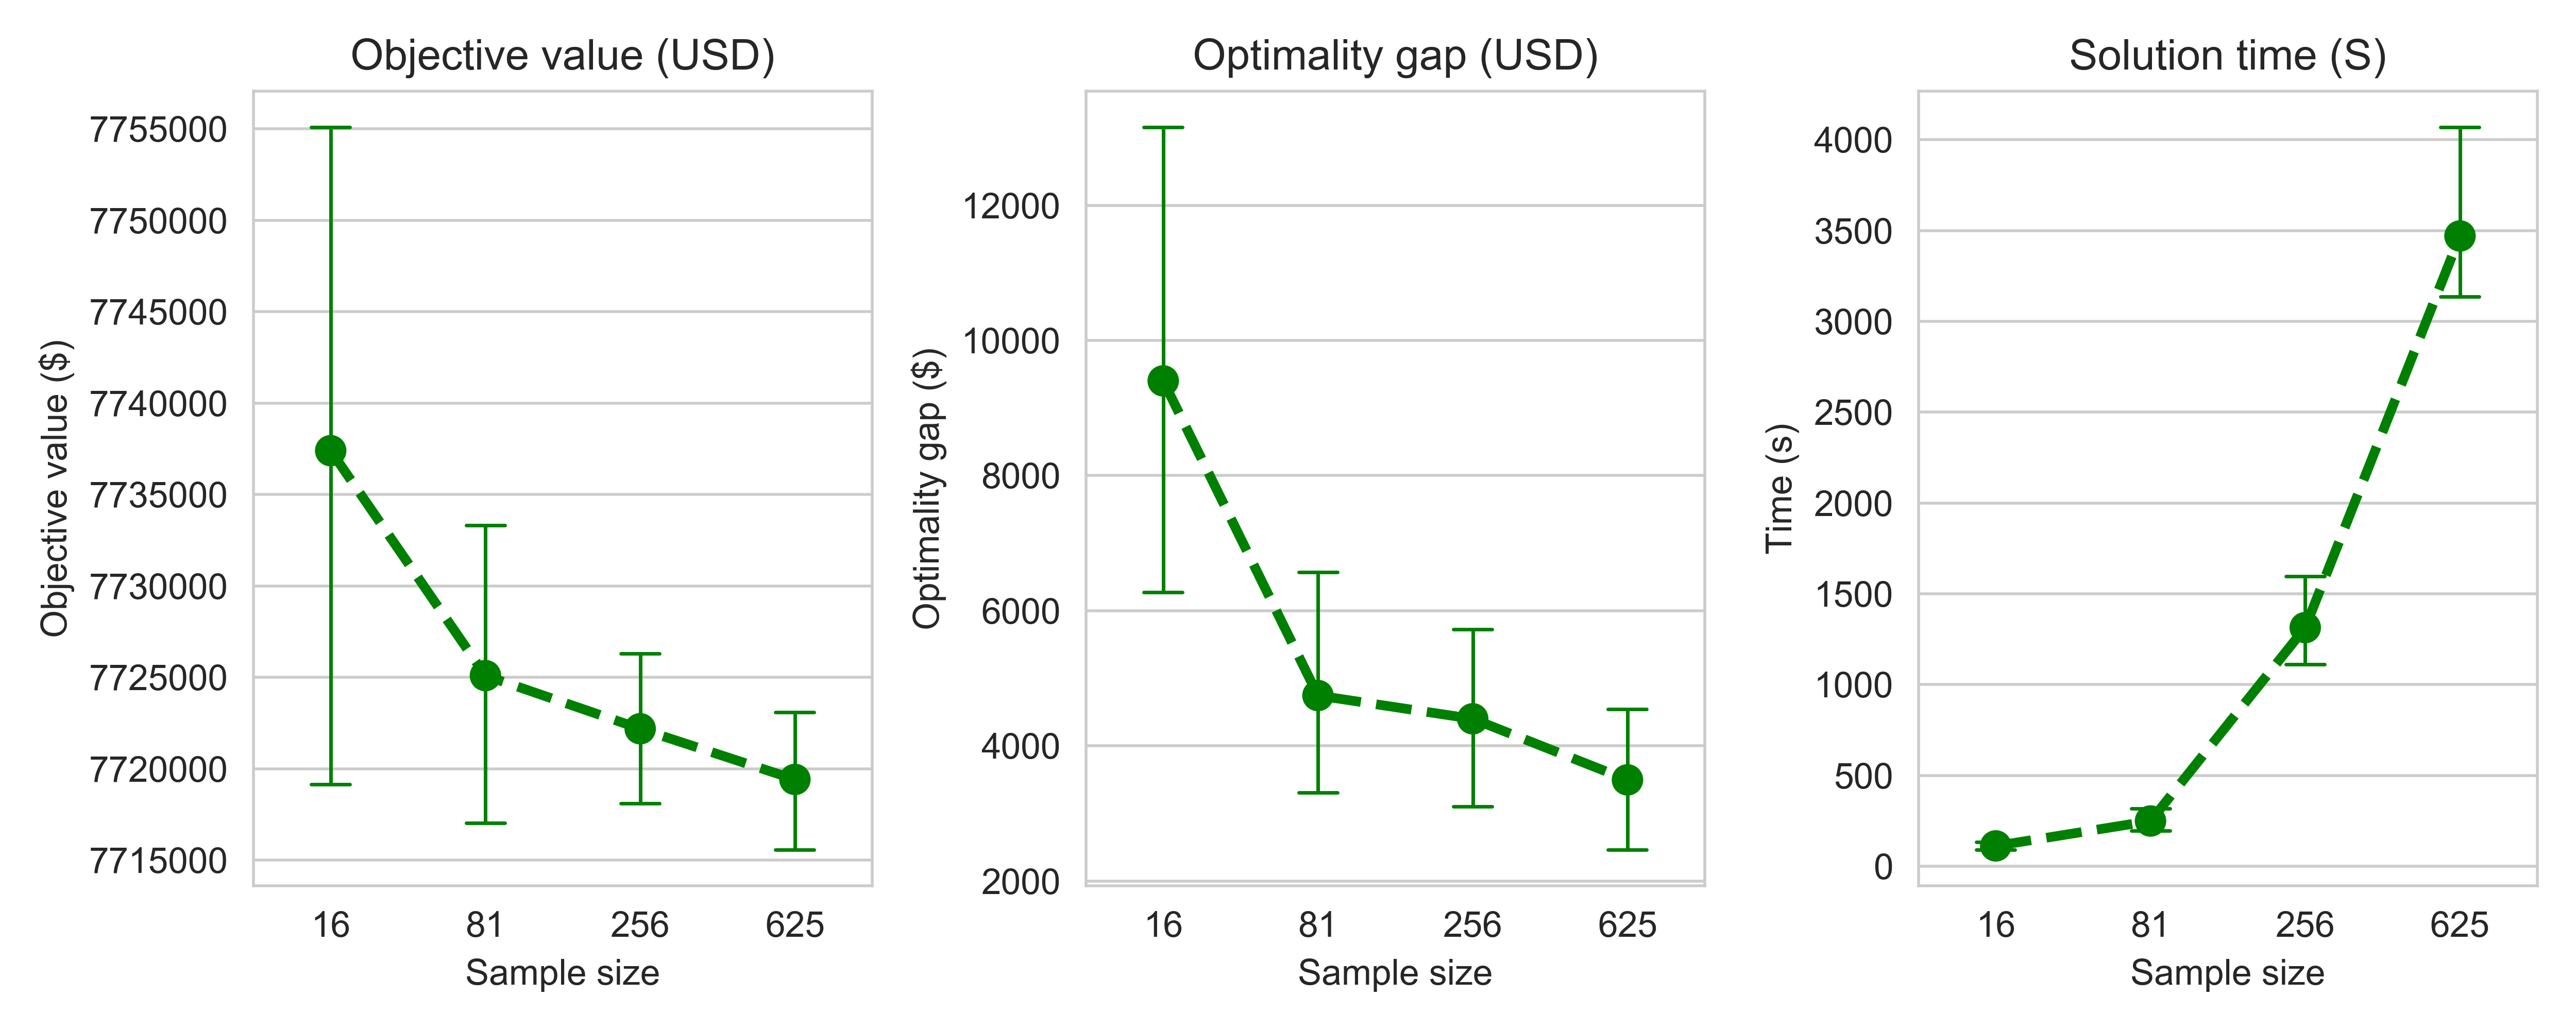
\includegraphics[width=1\linewidth]{sol_gap_time.png}
    \caption{Performance measurement of SAA for harvest scheduling. Error bars indicate 95\% confidence interval }
    \label{fig:saa_performance}
\end{figure}
 
 
% \begin{table}[!htb]
% \caption{Performance measurement of SAA for harvest scheduling for mild climate change}
% \label{tb:res_perf1}
% \centering\adjustbox{max width=\linewidth}{
% % \centering
% \begin{tabular}{lccccc}
% \toprule
% N   & Time (s) & Var.time & Obj.value (\$) & Gap (\$) & Err.Gap \\\hline
% 16  & 0.60 & 0.03     & 3,043,808    & 17,866    & 2,919          \\
% 81  & 2.11 & 1.17     & 3,026,288    & 3,530     & 1,063          \\
% 256 & 5.95 & 5.64     & 3,019,715    & 127      & 89 \\
% \bottomrule
% \end{tabular}
% }
% \end{table}


% \begin{table}[!htb]
% \caption{Performance measurement of SAA for harvest scheduling for severe climate change}
% \label{tb:res_perf2}
% \centering\adjustbox{max width=\linewidth}{
% % \centering
% \begin{tabular}{lccccc}
% \toprule
% N   & Time (s) & Var.time & Obj. value (\$) &        Gap (\$) &   Err.Gap \\\hline
% 16  & 0.66     & 0.11         & 2,942,789  & 141,618  & 9,170         \\
% 81  & 3.04     & 4.68         & 2,878,968  & 78,146   & 7,509         \\
% 256 & 25.43    & 1,093        & 2,597,222  & 41,566   & 4,923         \\
% 625 & 85.90     & 9,216        & 2,162,154  & 16,688   & 4,138 \\
% \bottomrule
% \end{tabular}
% }
% \end{table}

\subsection{Effect of sampling scheme on the optimality gap}\label{sec:sampl_scheme}

In this section, we test the effect of scenario generation scheme on the optimality gap. The scheme used to generate scenarios for the four stages is presented in Figure \ref{fig:gap_plot}. In the figure, the sampling scheme represents four digits corresponding to $N_1$, $N_2$, $N_3$ and $N_4$. For instance, \texttt{1155} means that $N_1=1, \; N_2=1, \; N_3=5$ and $N_4=5$ leading to 1*1*5*5=25 scenarios. This means that the schemes \texttt{1555} and \texttt{5551} lead to the same number of scenarios (125 scenarios). As we can see from Figure \ref{fig:gap_plot}, the optimality gap and its variability when $N_1$ = 1 is larger than when $N_1 > 1$. The lowest optimality gap is obtained with $N_1 = 3$. In general having higher values of $N_t$ for higher $t$ seems to be favorable. 
% Similar conclusions can be made when considering sampling schemes \texttt{5511} and \texttt{1155}.

\begin{figure}[!htb!]
    \centering
    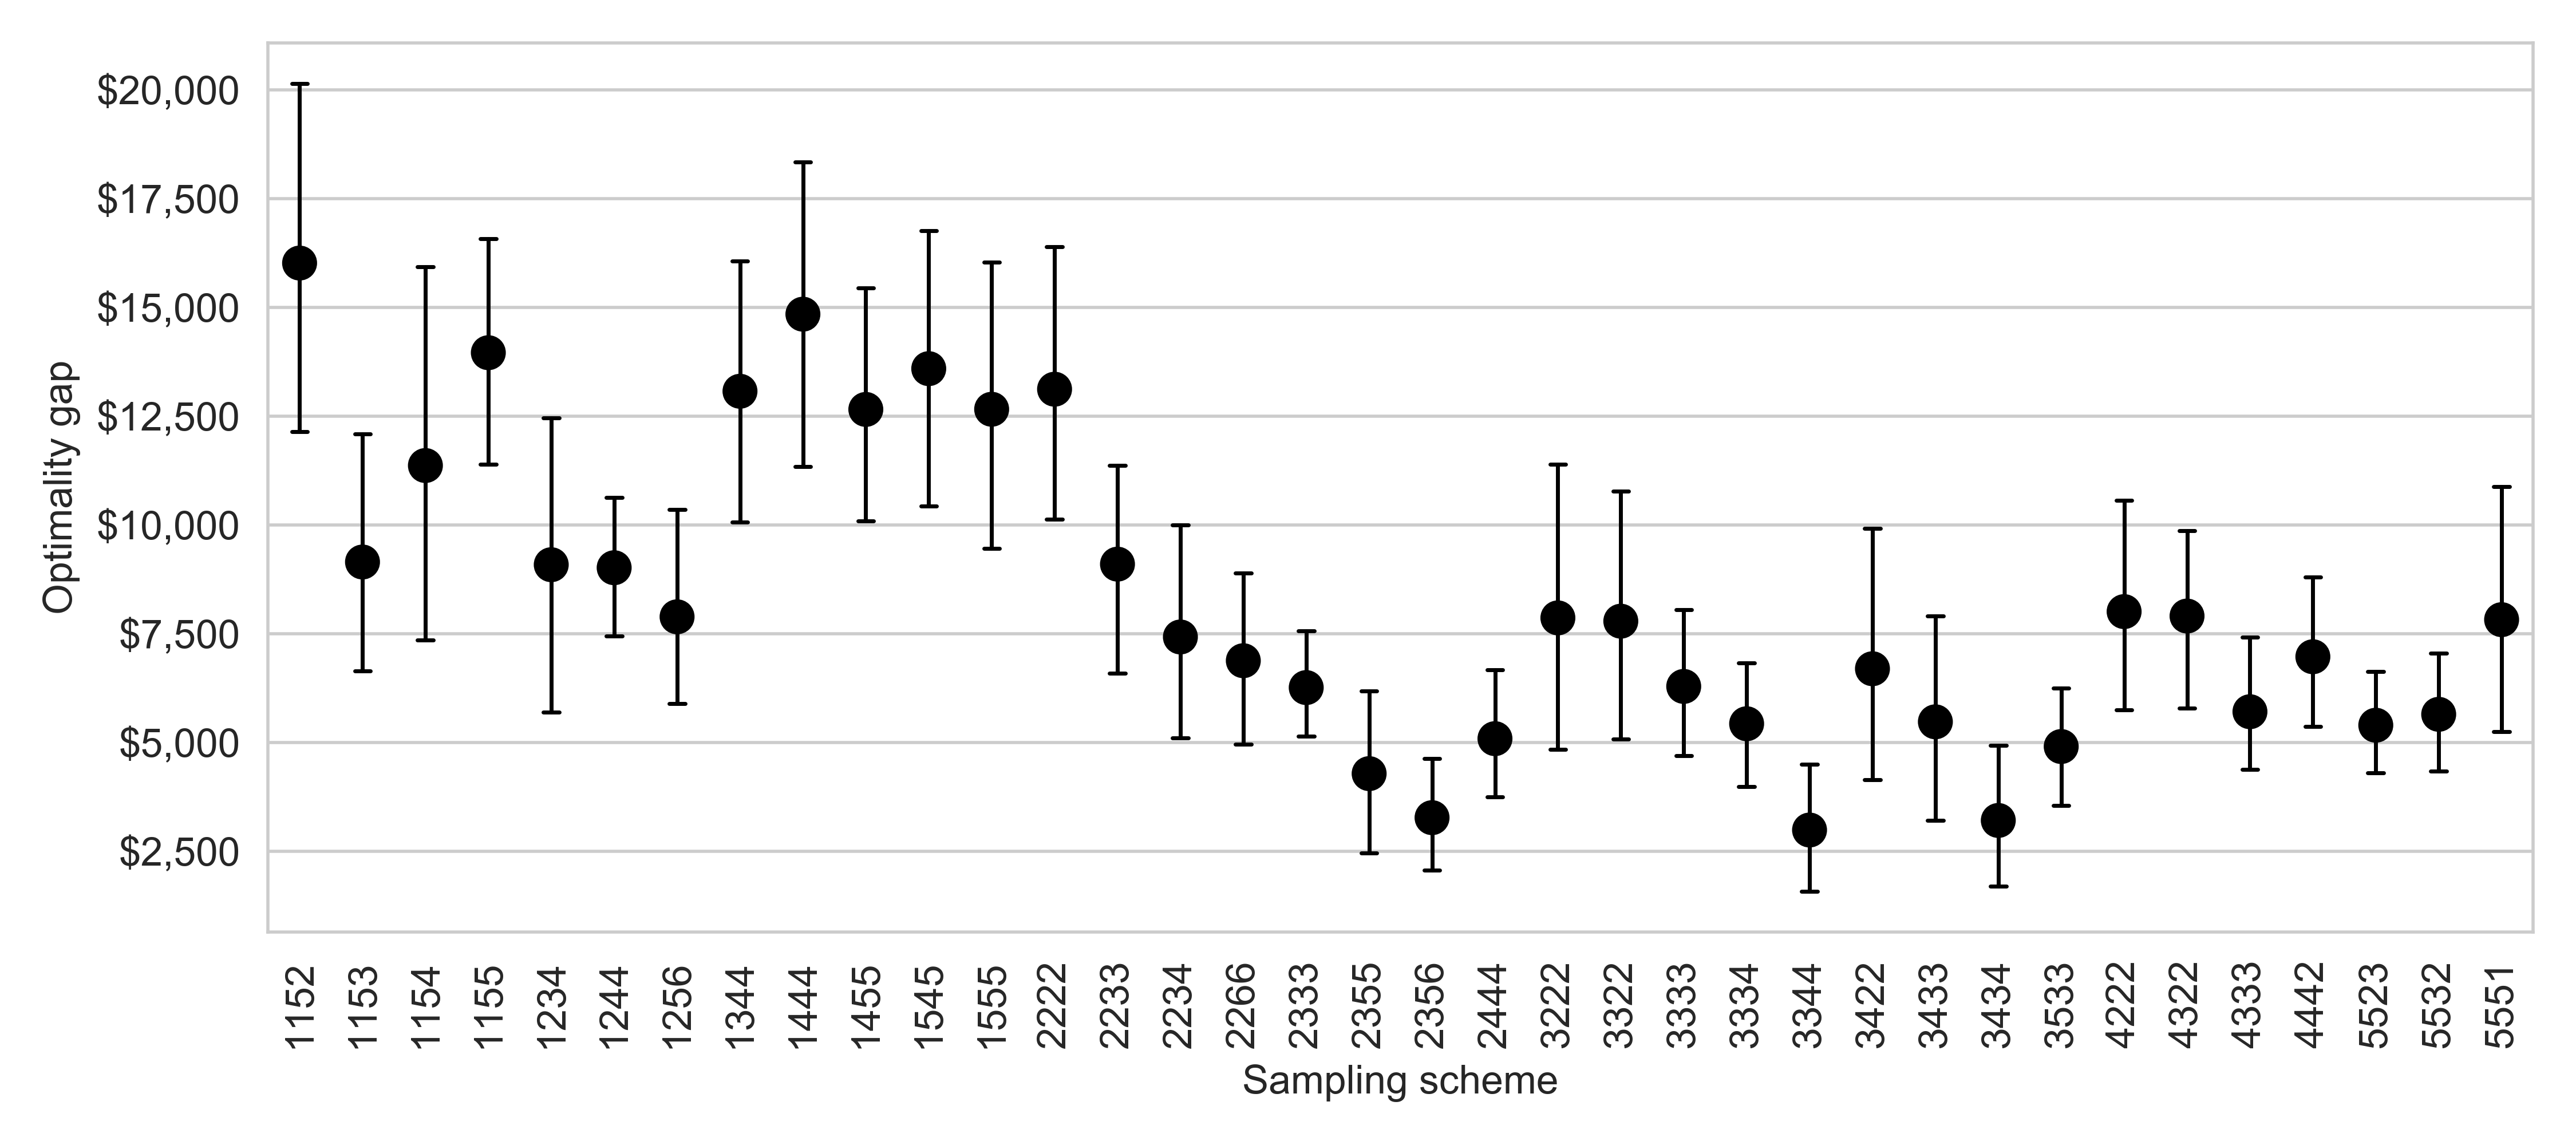
\includegraphics[width=1\linewidth]{cust_gaps_all.png}
    \caption{Change of optimality gap values due to the sample size and the configuration of the sampling scheme using severe climate change data}
    \label{fig:gap_plot}
\end{figure}

\subsection{Advantage of SAA in stochastic harvest scheduling over the deterministic approach}

The stochastic optimization solution allows to have superior solution in terms of NPV. In addition, it allows to have solutions that are robust (feasible) for a set of climate change scenarios that are not feasible if we implement here and now the deterministic solution (Table \ref{tab:cost_stochastic}). As the uncertainty on forest growth change magnitude increases, the value of stochastic solution increases as well. When we consider  $\epsilon=20$, out of 200 scenarios, 3 scenarios were infeasible.

\begin{table}[hbt!]
\caption{Value of the stochastic solution}
\label{tab:cost_stochastic}
\centering\begin{tabular}{lrrrrrr}
\toprule
$|\Omega|$ & $\epsilon$ & $z(\Bar{x})$ & $z(x^*)$   &  infeasible scen. & VSS      & VSS(bp) \\
\midrule
256                 & 1       & 7,775,108    &  7,782,679  & 0  & 7,571 & 9.96    \\
200                  & 20      & 7,160,950      & 7,256,069 & 3   & 95,119 & 132.83   \\
200                  & 40      &  4,940,204 &	6,737,368	& 60 & 1,797,163    &  3,637.83    \\
% 16                  & 50      &   -    &    -       & 10     &    -      &  -   \\
\bottomrule      
\end{tabular}\\
% N. Inf= number of scenarios infeasible when we implement the deterministic solution in the first stage.
\end{table}



\section{Discussion and conclusions} \label{sec:conclusion}

Climate change is a serious issue in forest management planning. In a study conducted in Norway, the majority of forest managers showed the importance of addressing climate change in forest planning \citep{Heltorp2018}. Several researchers conducted similar studies in different ecosystems and reached analogous results \citep{Scheller2018, Liu2020}. To ensure the sustainability of forest resources, forest managers need to incorporate forest growth uncertainty in harvest scheduling models. In this work, we formulated a stochastic harvest scheduling model with forest growth uncertainty due to climate change and solved the model using sample average approximation (SAA). We tested the modeling and solution using climate change data transformed to forest growth change. We compared the robustness of the stochastic solution to the deterministic one by randomly generating  a set of scenario and comparing the expected NPV if we implement the stochastic solution and the NPV if we use the deterministic solution. 
The numerical results showed that SAA allows to have stochastic solutions that are close enough to the true optimal solution when the sample size is large enough. However, large sample size lead to an exponential increase of solution time. This pattern of the computational complexity growing exponentially with the sample size was previously suggested by \cite{Kleywegt2001}. 

One of the main limitation of the proposed method is the computation required in step d of the algorithm  presented in Figure \ref{fig:saa_flowchart}. As we discussed in the previous paragraph, the increase of the sample size leads to an exponential increase in solution time. It is therefore important to have a strategy that allows to reduce the sample size while producing solutions that allow the convergence of SAA solutions to the true optimal solutions. Our tests suggest that with the appropriate sampling scheme, it is possible to reach convergence with smaller sample sizes. For instance, the sampling schemes  \texttt{2356} and \texttt{3344} yielding  sample sizes of 180 and 144, respectively, have smaller optimality gaps and variances compared to a sample size of 625 which stemmed from a sampling scheme of \texttt{5555}. 
In conclusion, when we adopt the adequate sampling strategy that allows to sufficiently explore the first stage and generate large samples for future stages, we can limit the number of scenarios necessary for the SAA solution to converge to the true  optimal solution. 

The proposed model not only allows the managers to make intelligent decision now, but also allows the preservation of forest resources that take time to replenish once depleted. Indeed, the stochastic solution is robust to different climate scenario whereas, the deterministic one is infeasible to many of the tested climate scenarios. These results are in line with the ones obtained by \cite{Alvarez-Miranda2018, Garcia-Gonzalo2020}. The infeasibility of the deterministic solution stems mainly from the fact that the wood flow constraints are violated due to an intensive harvest in early periods. 

In addition, the  solution method proposed in this paper is easy to develop and implement  by many forest managers. Unlike the methods used in \cite{Garcia-Gonzalo2016, Garcia-Gonzalo2020} that require to know the probability distribution of the random parameter, SAA does not require such information. The method relies on the fact that if the sample size is large enough, then the sample statistics  will approximate those of the actual population. The method is also suitable for many applications where the objective function cannot be computed in a closed form such as the so-called black-box optimization problems \citep{Kim2011} and the stochastic knapsack problem \citep{Kleywegt2001}. In forestry, this method is well suited for harvest scheduling problem with wood price and demand uncertainties because we can extract samples from historical demand and price without the need to model the price like done in \cite{Rios2016, Alonso-Ayuso2018}.
Compared to stochastic programming which require the so-called non-anticipativity constraints \cite{Bagaram__AD, Garcia-Gonzalo2020}, SAA model is relatively smaller in terms of number of constraints (and possibly in terms of number of variables, depending on the formulation) since it does not require such constraints.

Regarding climate change data, we  used the information of climate change forecast with statistical models developed in \cite{Latta2009}. Unlike the data from \cite{Garcia-Gonzalo2016,Alvarez-Miranda2018, Garcia-Gonzalo2020}, which originated from a process-based modeling, statistical models of forest growth under climate change are much more common (for e.g \cite{Elli2020}). Hence, the method developed in this study can easily be extended to other forest systems. Moreover, it is straight forward to translate forecast of precipitation, air moisture and temperature into forest growth compared to processed-based models which require the expertise in plant biology.

Finally, this research can be extended by considering other sources of uncertainty such as the price of wood, or the demand of forest products. In this research we assumed that climate change does not lead to species transition. In some cases, one might need to consider the species shift because of climate change. It would be interesting to include this information in the decision-making process and provide to forest practitioners a range of options when implementing harvest scheduling plans and the choice of species for regeneration.

\vspace{6pt} 



%%%%%%%%%%%%%%%%%%%%%%%%%%%%%%%%%%%%%%%%%%
\funding{This research received funding of Precision Forestry Cooperative of the School of Environmental and Forest Sciences, University of Washington 
% or ``This research was funded by NAME OF FUNDER grant number XXX.'' and  and ``The APC was funded by XXX''. Check carefully that the details given are accurate and use the standard spelling of funding agency names at \url{https://search.crossref.org/funding}, any errors may affect your future funding.
}

%%%%%%%%%%%%%%%%%%%%%%%%%%%%%%%%%%%%%%%%%%
% \acknowledgments{In this section you can acknowledge any support given which is not covered by the author contribution or funding sections. This may include administrative and technical support, or donations in kind (e.g., materials used for experiments).}

%%%%%%%%%%%%%%%%%%%%%%%%%%%%%%%%%%%%%%%%%%
\conflictsofinterest {The authors declare no conflict of interest.} 



%----------------------------------------------------------------------------------------
%% optional
\appendixtitles{yes} %Leave argument "no" if all appendix headings stay EMPTY (then no dot is printed after "Appendix A"). If the appendix sections contain a heading then change the argument to "yes".
\appendix
% \section{}
% \unskip

\section{Deterministic harvest scheduling model} \label{app:det_harv}

The objective function (\ref{eq:obj_2_det}) is to maximize the net present value from forest harvest. This objective function includes the cost of harvest and re-plantation for each forest unit. In addition, this objective function accounts for the value of the stands that are not harvested during the planning horizon because those stand have a monetary value. Constraint set (\ref{eq:one_harvest_det}) imposes that if a stand is harvested now, then it cannot be harvested in subsequent years. In other words a forest unit can only be harvested once during the whole planning horizon. The use of $n_s$ variables is to account the stands that are not scheduled for harvest in the whole planning horizon.
Constraint set (\ref{eq:compute_v_others_det})  compute the volume of wood harvested  now and in the future periods during the planning horizon, respectively.
Constraint sets  (\ref{eq:vol_flu_low_det}) and  (\ref{eq:vol_flu_high_det}) impose that the volume fluctuation between two consecutive stages should be within a fixed lower and upper bounds, respectively. These set of constraints are also known as even flow constraint since they ensures that the exploitation of forest resources is evenly distributed in time. Even with constraint sets  (\ref{eq:vol_flu_low_det}) and  (\ref{eq:vol_flu_high_det}), there is a possibility that the volume harvested declines with time. Hence volume at $t=4$ is much lower than volume at $t=0$, for instance. To attenuate this effect, we impose supplementary wood flow constraints which are constraint sets (\ref{eq:vol_flu_low2_det}) and  (\ref{eq:vol_flu_high2_det}). These two set of constraints impose flow restriction between two non consecutive stages.
Constraint set (\ref{eq:age_end_det}) states that the age of the forest at the end of the planning horizon should be greater or equal to the current age of the forest. This constraint is a proxy for sustainability; it ensures that forest resources are not depleted during the planning horizon.  Finally, the definition of the variables are given in (\ref{eq:var_definition_det}).

\begingroup
\allowdisplaybreaks
\begin{align}
    & \max \; \sum_{s =1 }^{|\mathcal{S}|} \Bigg[ \sum_{t=0}^{{T}} r_{st}x_{st}  + r_{s0} w_s \Bigg]\label{eq:obj_2_det}\\
& \text{subject to} \nonumber\\
    & n_s + \sum_{t=0}^T x_{st} = 1 \quad \quad  s=1,\dots, |\mathcal{S}| \label{eq:one_harvest_det}\\
    % & \sum_s x_s v_s = H_0 \label{eq:compute_v0}\\
    & \sum_s v_{st} x_{st} = H_{t} \quad \quad   t = 0, \dots, T \label{eq:compute_v_others_det}\\
    & H_t^{i} \le \alpha H_{t-1} \quad \quad   t=1, \dots, T \label{eq:vol_flu_low_det}\\
    & H_t^{i} \ge \beta H_{t-1} \quad \quad  t=1, \dots, T \label{eq:vol_flu_high_det}\\
     & H_t \le \gamma H_{t-2} \quad \quad   t=2, \dots, T \label{eq:vol_flu_low2_det}\\
    & H_t^{i} \ge \lambda H_{t-2} \quad \quad  t=2, \dots, T \label{eq:vol_flu_high2_det}\\
    & \sum_{s\in \mathcal{S}}a_s\Bigg[\sum_{t=0}^{\mathcal{T}} age_{st} x_{st} + age_{s0}w_{s}\Bigg] \ge \sum_s a_s age_{s.} \label{eq:age_end_det}\\
    & w_s \in \{0, 1\}, \; \forall s, \; x \in \{0, 1\}^{|\mathcal{S}| \times T+1}, \; \; H_{t} \ge 0 \quad \forall t \label{eq:var_definition_det}
\end{align}
\endgroup


\reftitle{References}
% \bibliographystyle{elsarticle-harv} 
\bibliography{all_references}

\end{document}

